\documentclass{panikzettel}

\title{Panikzettel EMS}
\author{Kevin Conrads}

\usepackage{listings}
\lstset{basicstyle=\ttfamily\footnotesize,breaklines=true}

\begin{document}

\maketitle

\tableofcontents

\section{Einleitung}
Dieser Panikzettel für das Fach ``Einführung in Management Science: Desgin und Analyse von Algorithmen'', gehalten im WS19/20 von Prof. Peis, ist ein freiwilliges Projekt, dass ich parallel zu meiner Tutortätigkeit in diesem Fach erstellt habe. Die Struktur folgt dabei in der Reihenfolge den Vorlesungsthemen, kann jedoch an sinnvollen Stellen davon abweichen.

Dieses Dokument hat \emph{nicht} zum Ziel, alleinige Ressource zum Lernen und Verstehen des Vorlesungsstoffes zu sein, sondern eine begleitende bzw. ergänzende Rolle zu den Materialien aus der Vorlesung und Übung einzunehmen. Trotz größter Sorgfalt können Fehler, die Inhalt, Form, Notation, etc. betreffen, nicht ausgeschlossen werden. Es liegt daher in der Verantwortung des/der Leser/Leserin, sich im Zweifel mit den betreffenden Lehrmaterialien der Vorlesung auseinanderzusetzen. Außerdem hafte ich nicht für falsche Antworten in z.B. der Klausur, aufgrund der Informationen in diesem Dokument getätigt wurden. 

Eltern haften für ihre Kinder.

\vspace{-0.5\baselineskip}
{\small{}
	\paragraph{Hinweis:}
	Das Latex-Template für diesen Panikzettel sowie das Konzept ``Panikzettel'' an sich sind übernommen bzw. angelehnt an das \href{https://git.rwth-aachen.de/philipp.schroer/panikzettel}{Panikzettel-Projekt}.

\section{Stabile Matchings}

\begin{halfboxl}
	\vspace{-\baselineskip}
	\begin{defi}{Stable Marriage Problem}
	Das Stable Marriage Problem beschreibt, wie eine Menge von Männern und eine gleichgroße Menge von Frauen miteinander verlobt (\emph{gematched}) werden sollen, so das keiner einen Anreiz zu einem Seitensprung hat.\\
	
	\begin{itemize}
		\item Es gibt eine Menge an $n$ Männern und eine Menge an $n$ Frauen
		\item Jeder Mann listet die Frauen nach absteigender Präferenz
		\item Jede Frau listet die Männer nach absteigender Präferenz
		\item Gesucht ist ein Arrangement an $n$ Hochzeiten, das heißt ein \emph{perfektes Matching}
		\item Das Matching soll möglichst stabil sein: Keiner sollte einen Anreiz zu einem Seitensprung haben
	\end{itemize}
	\end{defi}
\end{halfboxl}%
\begin{halfboxr}
	 \vspace{-\baselineskip}
	Graph-Beispiel für das Stable Marriage Problem:\\
	
	\begin{center}
	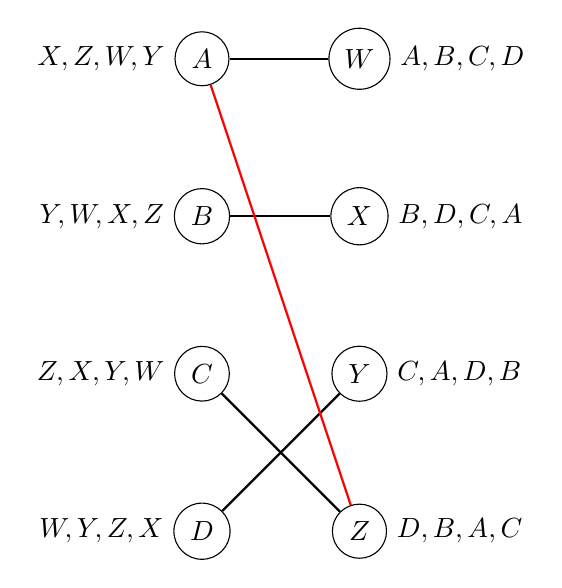
\begin{tikzpicture}
	\node[draw,circle,minimum size=5mm, label = left:{$X,Z,W,Y$}] (A) at (0,0) {$A$};
	\node[draw,circle,minimum size=5mm, label = left:{$Y,W,X,Z$}] (B) at (0,-2) {$B$};
	\node[draw,circle,minimum size=5mm, label = left:{$Z,X,Y,W$}] (C) at (0,-4) {$C$};
	\node[draw,circle,minimum size=5mm, label = left:{$W,Y,Z,X$}] (D) at (0,-6) {$D$};
	
	\node[draw,circle,minimum size=5mm, label = right:{$A,B,C,D$}] (W) at (2,0) {$W$};
	\node[draw,circle,minimum size=5mm, label = right:{$B,D,C,A$}] (X) at (2,-2) {$X$};
	\node[draw,circle,minimum size=5mm, label = right:{$C,A,D,B$}] (Y) at (2,-4) {$Y$};
	\node[draw,circle,minimum size=5mm, label = right:{$D,B,A,C$}] (Z) at (2,-6) {$Z$};
	%\foreach \X [count=\Y from 2] in {1, ..., 3}{
	%	\draw[-] (\X) -- (\Y);
	%}
	\draw[thick] (A) -- (W);
	\draw[thick] (B) -- (X);
	\draw[thick] (C) -- (Z);
	\draw[thick] (D) -- (Y);
	\draw[thick,red] (A) -- (Z);
	\end{tikzpicture}
	
	Hier liegt ein instabiles Matching vor: $\{A,Z\}$ sind unzufrieden mit der Partnerwahl; sie finden sich gegenseitig besser als ihre jetzigen Partner und hätten damit Anlass für einen Seitensprung.
	\end{center}
\end{halfboxr}

%\vspace{0.5cm}

\begin{halfboxl}
	\vspace{-\baselineskip}
	\begin{defi}{Matchings in Graphen}
	Sei $G = (V,E)$ ein ungerichteter Graph\\
	
	\begin{itemize}
	\item Eine Teilmenge $M$ der Kanten wird Matching gennant, wenn keine zwei Kanten in $M$ einen gemeinsamen Endknoten haben.
	
	\item Die Kardinalität $|M|$ (Anzahl der Kanten in $M$) eines Matchings $M$ ist nie größer als $\frac{|V|}{2}$
	
	\item Ein Matching $M$ mit $|M| = \frac{|V|}{2}$ heißt \emph{perfekt}
	
	\end{itemize}
	\end{defi}
\end{halfboxl}%
\begin{halfboxr}
	\vspace{-\baselineskip}
	\begin{defi}{Bipartite Graphen}
	Ein ungerichteter Graph $G = (V,E)$ heißt \emph{bipartit}, wenn sich die Knotenmenge $V$ so in zwei Hälften aufteilen lässt, dass\\
	
	\begin{itemize}
		\item $V = L \cup R$ (jeder Knoten ist entweder in $L$ oder in $R$),
		\item $L \cap R = \emptyset$ (kein Knoten liegt in beiden Mengen) und 
		\item das jede Kante einen Endknoten in $L$ und einen in $R$ besitzt.
	\end{itemize}
	\end{defi}
\end{halfboxr}

\begin{defi}{Blockierende Kante und Stabiles Matching}
	Eine Kante ${u,v}$ heißt \emph{blockierend} (für ein Matching $M$), wenn der Knoten $u$ den Knoten $v$ gegenüber seinem jetzigen Partner präferiert und umgekehrt.
	
	Ein Matching $M$ ist \emph{stabil}, wenn es keine blockierende Kante im Graphen gibt.
	
	\textit{(Im Beispiel Graph oben ist die rot gezeichnete Kante $\{A,Z\}$ eine blockierende Kante für das Matching.)}
\end{defi}
\section{Sortieren}

\section{Laufzeit}

\section{Interval-Scheduling und Partitioning}

\section{Graphentheorie}

\section{Minimale Spannbäume}

\section{Einführung in Spieltheorie}

\section{Networkflow und Project Selection}

\section{Matching Markets}

\section{Prolog}

\end{document}